\chapter{Prior Work}

%\begin{shadequote}
%If I have seen further it is by standing on the shoulders of giants.\par\emph{Isaac Newton}
%\end{shadequote}

%cut out up to we?
\begin{shadequote}
Bernard of Chartres used to say that we are like dwarfs on the shoulders of giants, so that we can see more than they, and things at a greater distance, not by virtue of any sharpness of sight on our part, or any physical distinction, but because we are carried high and raised up by their giant size.\par\emph{John of Salisbury}
\end{shadequote}


\section{Background and Theory}
\subsection*{Ecotype Model of Bacterial Species}
An ecotype is defined as a bacterial cluster with individuals that are ecologically similar to one another, so much so that genetic diversity within the ecotype is limited by a cohesive force, either periodic selection or genetic drift, or both~\cite{cohan2007systematics}.
By linking species and ecological niche we take advantage of the natural clustering of organisms according to environmental resources.
Since these clusters are evolving together we do not need to utilize morphological differences and can instead use a molecular approach for demarcation.

Ecotypes have all the dynamic properties of a species, each is a cohesive group, different ecotypes are irreversibly separate because they are out of range of one another's cohesive force, and because recombination is too rare to prevent their adaptive divergence; they are by definition ecologically distinct, which allows them to coexist into the future~\cite{cohan2007systematics}.
Or, essentially the fundamental unit of microbial ecosystems.
Efforts to define prokaryotic species according to these properties have differed most profoundly in the forces of cohesion thought to be most important for prokaryotic species~\cite{cohan2008origins}.
ES uses one model in particular to understand ecotype bacterial speciation.

\subsection*{Stable Ecotype model}

\begin{figure}[h!]
% \caption{Three classes of mutation and recombination events that determine ecotype diversity in bacteria. Circles represent different genotypes, and asterisks adaptive mutations. (A) Periodic selection purges diversity. (B) Ecotype formation creates diversity. (C) Extinction events SHOULD I CUT THIS OUT?.(reprinted from \protect\cite{cohan2007systematics})}
 \centering
 \label{fig:StableEvents}
 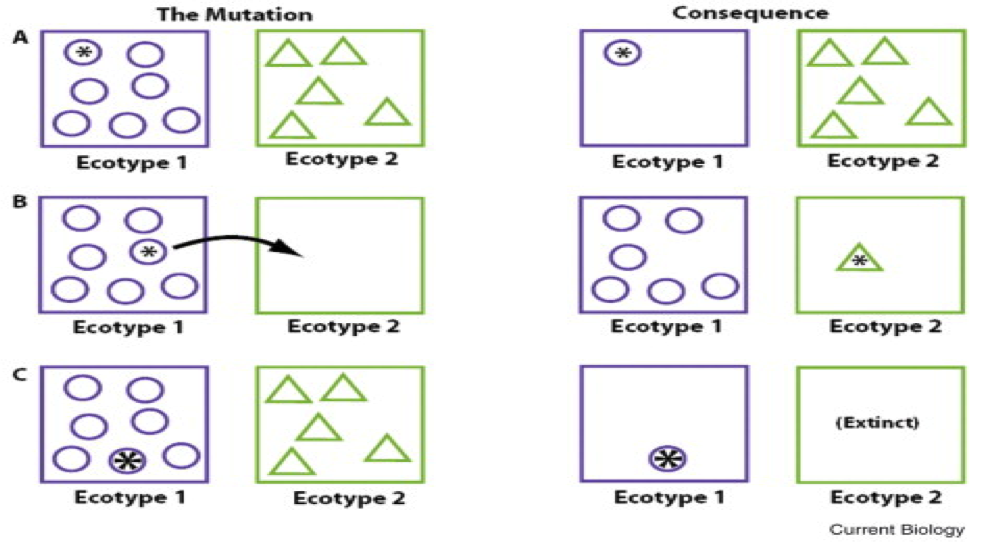
\includegraphics{images/StableEcotypeEvents-CH2}
 \caption{Three classes of mutation and recombination events that determine ecotype diversity in bacteria. Circles represent different genotypes, and asterisks adaptive mutations. (A) Periodic selection purges diversity. (B) Ecotype formation creates diversity. (C) Extinction events. (reprinted from \protect\cite{cohan2007systematics})}
\end{figure}

In the Stable Ecotype model ecotypes are created and extinguished at a very low rate, and during its long lifetime an ecotype is recurrently purged of its diversity by periodic selection events~\cite{cohan2007systematics}.
Ecotypes are formed rarely enough so that they can accumulate its own set of unique mutations while diversity is purged, yielding a correspondence between ecotypes and sequence clusters for any gene shared among ecotypes~\cite{cohan2008origins}.
This fact, hinted at earlier, is what allows ES to identify separate ecotypes based on environmental function without knowledge of particular phenotypic mutations.
Diversity quashing events are referred to as periodic selection events, see Figure~\ref{fig:StableEvents}a.
An individual of a ecotype acquires a mutation that improves its fitness within that ecological niche, which results in a diversity purge, due to low recombination rates in bacteria, where other organisms in the ecotype without the adaption become extinct.
Genetic drift is another event that results in diversity purges, however it is normally quite rare.

%Describes relationship of periodic selection events and ecotype formation event
Early during speciation, a new ecotype's niche may rely on proportions of resources used and may be vulnerable to extinction by periodic selection caused by an adaptive mutation within the parental ecotype.
However, a single HGT event may transfer the adaptive mutation across ecotypes, and could thereby prevent extinction of one ecotype by another~\cite{cohan2008origins}.
In this case an ecotype formation event occurs, see Figure~\ref{fig:StableEvents}b.
The ecotype-transcending adaptation allowed an ecotype speciation event to occur. In the figure an individual of an ecotype developed an adaptation that went on to colonize a new niche creating a new ecotype.

Now we have an event to account for anagenesis, or accumulation of changes over time along a single lineage, referred to as periodic selection, and cladogenesis, or irreversible splitting of lineages, referred to as ecotype formation.
To complete the dynamics of the Stable Ecotype model, extinction events are also possible, see Figure~\ref{fig:StableEvents}c.
An ecotype, obviously, can go extinct.
Previous work done in the Cohan lab was done to develop an algorithm based on the Stable Ecotype model, which eventually became known as Ecotype Simulation.


\section{The Algorithm}

\begin{SCfigure}
 \caption{ The Stable Ecotype model, in which ecotype formation is relatively rare, and periodic selection events frequently purge all diversity from within each ecotype. This model predicts a one-to-one correspondence between sequence clusters and ecotypes. (reprinted from \protect\cite{cohan2008origins}) }
 \centering
 \label{fig:StableTree}
% 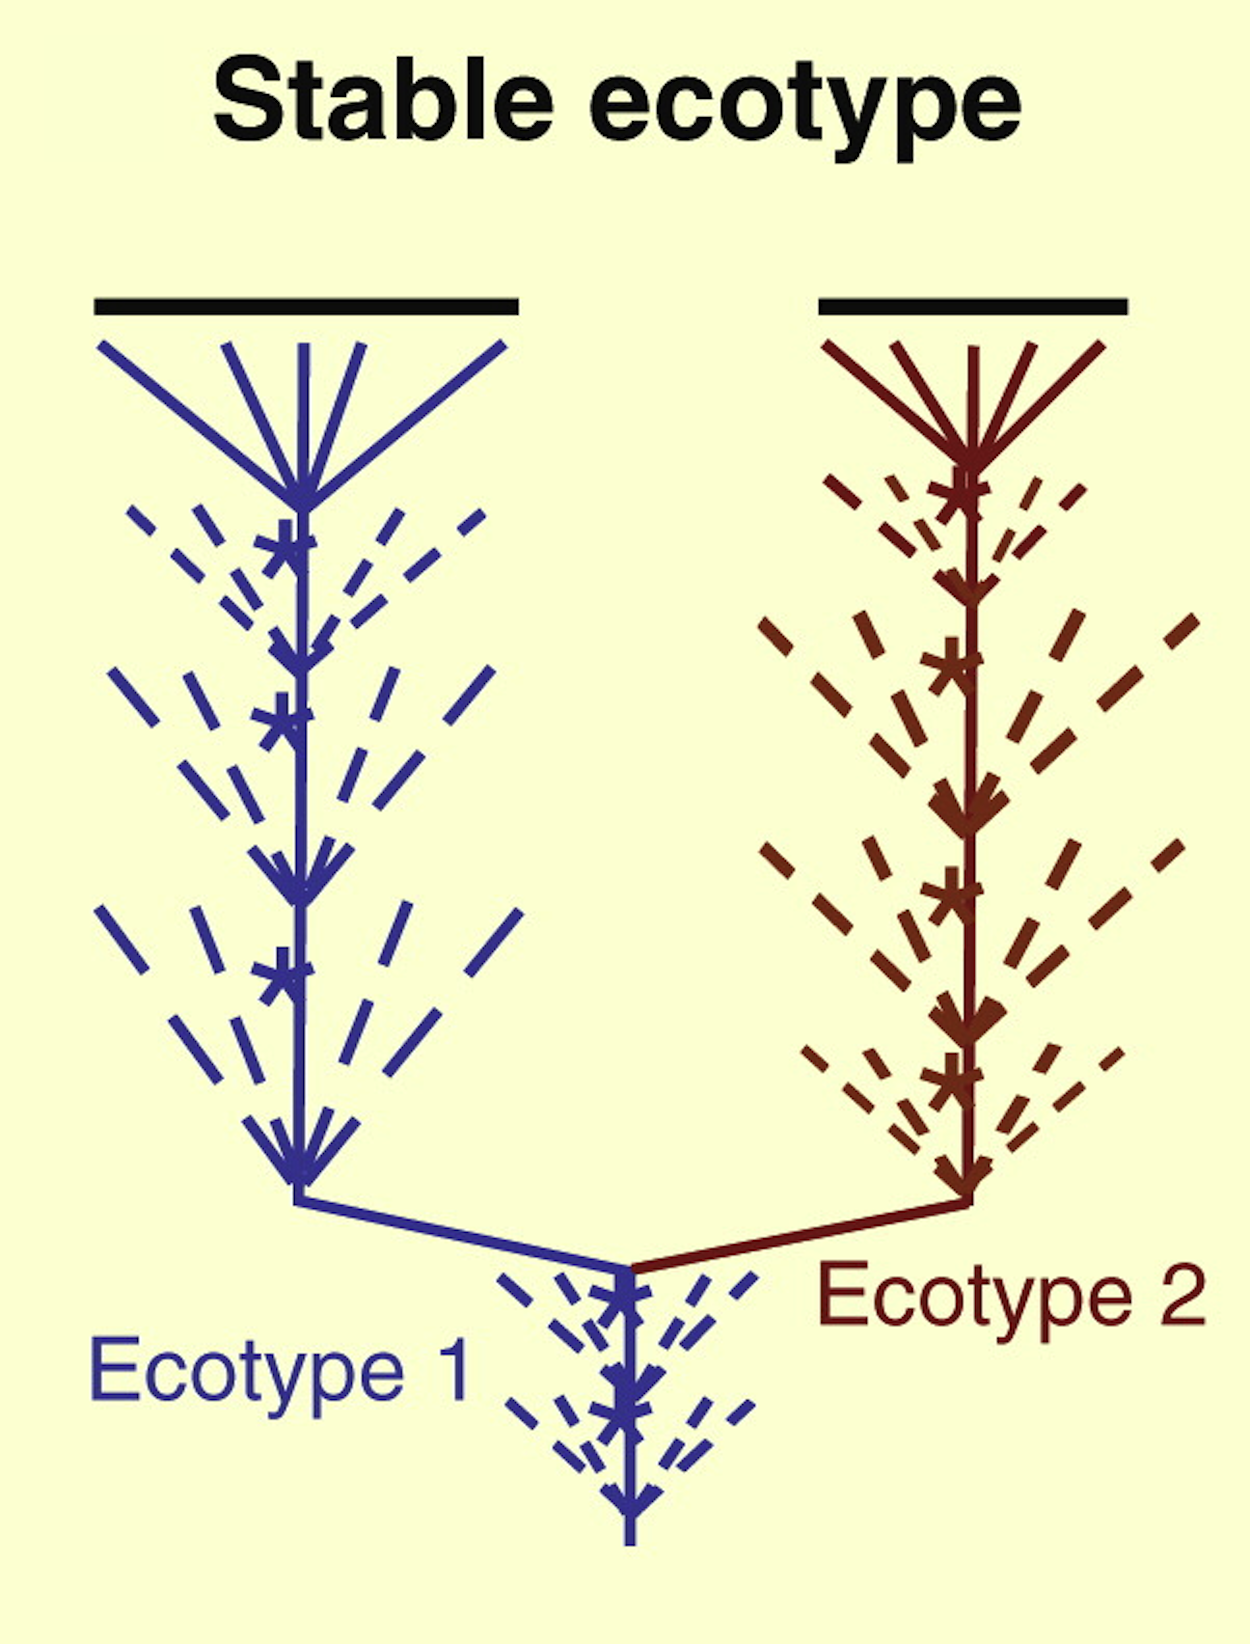
\includegraphics{images/StableTree-CH2}
 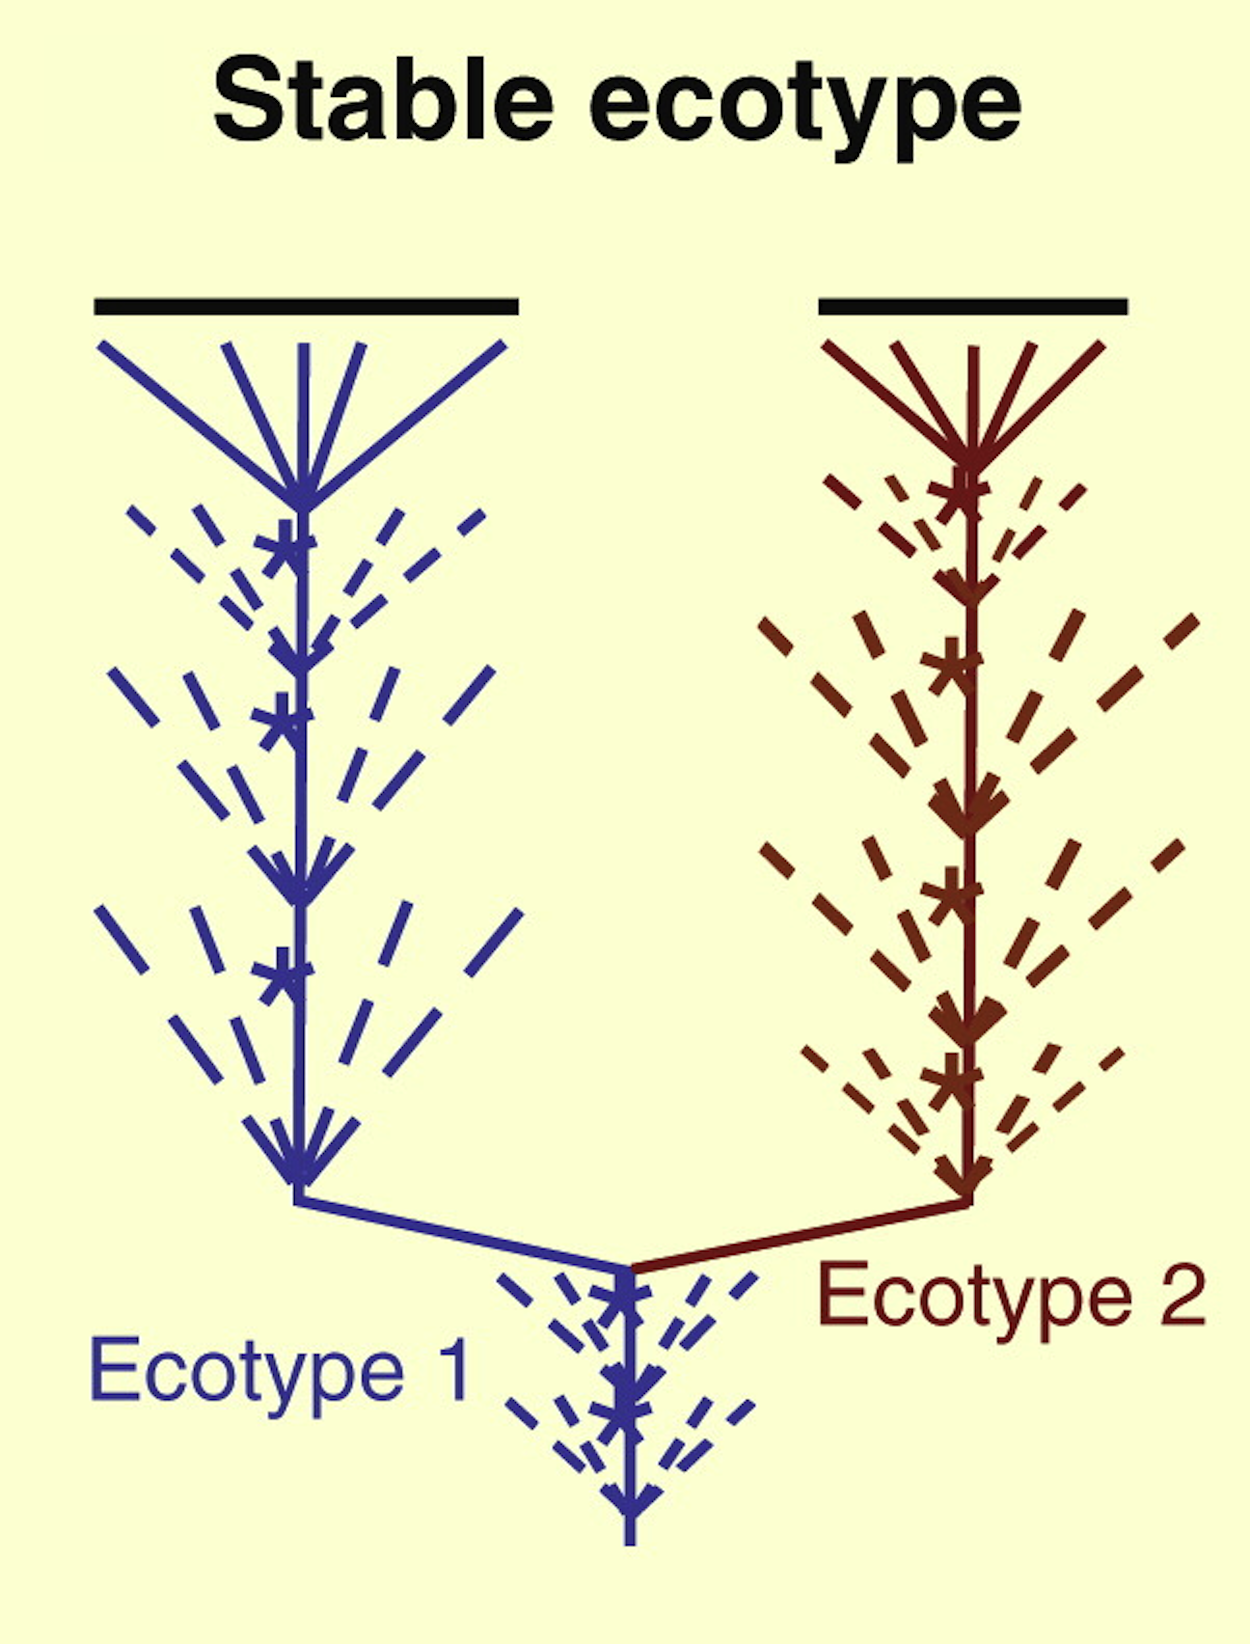
\includegraphics[width=0.5\textwidth]{images/StableTree-CH2}
\end{SCfigure}

Utilizing the premises established in the Stable Ecotype model we produce a tree in most cases similar to the one represented in Figure ~\ref{fig:StableTree}. 


Here I'll go over the process in non-system specific way. Make phylogeny based on distances. Then we want to find the parameters that describe the sequence identity graph. Then describe why these parameters are relevant and the power they give us. Allow us to pick at which point we pass diversity between different species groups and diversity within a species group.



\section{Ecotype Simulation}

\begin{figure}[h!]
 \centering
 \label{fig:Binning}
 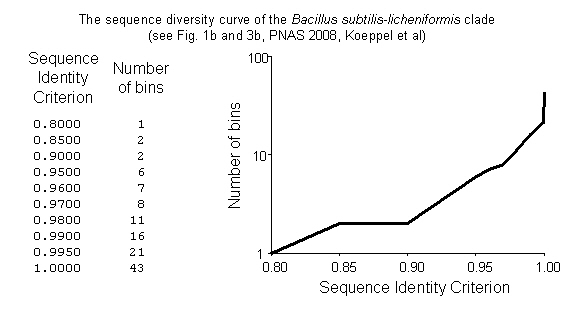
\includegraphics{images/Binning-CH2}
 \caption{An example output of information from the initial binning of wild-type sequences. (adapted from \protect\cite{koeppel2008identifying}) }
\end{figure}

%EDIT CAPTION
\begin{figure}[h!]
%The program begins with a ``backward'' simulation that stochastically produces a phylogenetic representation of the history of the community, establishing nodes of coalescence of lineages (due to PS, EF, or D; indicated by gray circles) and time between nodes (t1, t2, etc.); this phylogeny is then taken as a scaffold for the forward simulation. The purpose of the forward simulation is to produce mutational nucleotide substitutions throughout the history of the clade, according to the phylogenetic scaffold. To begin a simulation, a set of v contemporary organisms (representing the ? organisms sampled from nature) are distributed randomly (according to the canonical lognormal distribution) among n ecotypes (here, ? = 14 and n = 3). Working backward from the ? organisms in the present, the processes of EF, PS, and D occur stochastically in time according to their respective rates ($\Omega$, $\sigma$, and d). For each such event, one or more lineages coalesce into a single ancestral lineage, as described in SI. Note that in the backward-looking view of the coalescence formulation, each PS appears as a coalescence event, in which all lineages after the PS coalesce into the survivor of the PS event. Likewise, each D event appears in this backward-looking view as the coalescence of a pair of lineages within an ecotype (e.g., two contemporary lineages coalesce into lineage D1 to reflect the increased representation of lineage D1 after the random loss by drift of lineage D2). Because $\Omega$ is the net rate of EF events, taking into account extinction, we include in the simulation only those EF events resulting in ecotypes that survive into our contemporary sample. The backward phase of the simulation ends when all of the branches have coalesced into a single node; this represents the most recent common ancestor of all of the sampled organisms. Then the forward simulation begins when a sequence (of the same length as the observed sequence data) is assigned to this most recent common ancestor. Nucleotide substitutions then occur stochastically, going forward in time, between each pair of nodes in the phylogeny derived from the backward simulation, according to the time between the events determining the nodes. This generates a matrix of pairwise sequence divergence between all v contemporary organisms for a simulation replicate, from which a clade sequence diversity curve is calculated; the simulated clade sequence diversity curve is then compared against the observed clade sequence diversity curve (see SI).%
  \centering
  \label{fig:SpeciationGraph}
   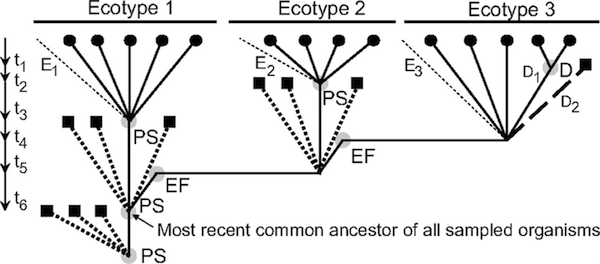
\includegraphics{images/Speciation-CH2}
   \caption{A phyolgeny representation of the ecotype simulation algorithm. The algorithm simulates the evolutionary history of the organisms sampled from nature under different values for the net rate of ecotype formation (EF), rates of periodic selection (PS), drift (D), and the number of ecotypes in the sample. It only considers existing individuals (black circles) from non-extinct lineages represented by bold lines. Previously extinguished lineages, due to past PS or D events, are represented by dotted lines and squares. (reprinted from \protect\cite{koeppel2008identifying})}
\end{figure}

\begin{figure}[h!]
 \centering
 \label{fig:Flow}
 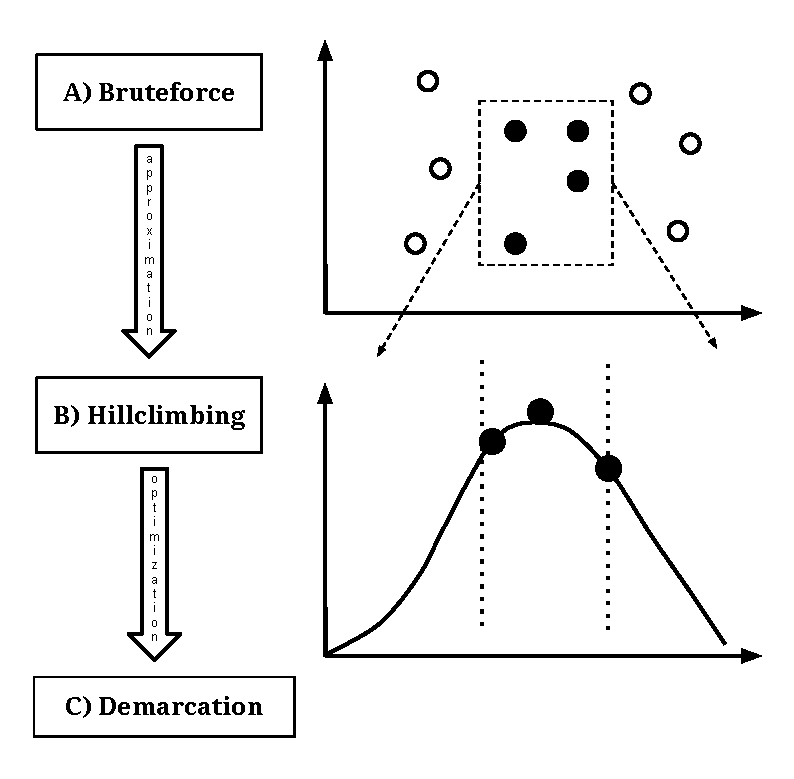
\includegraphics[scale=0.75]{images/ESFlow-CH2.pdf}
 \caption{This is the program call flow of ES. (figure created with help from Lingyuan Ke) }
\end{figure}

Here we can show how we attempt to implement this algorithm. Use system diagrams going from binning to brute force to hill climbing to automatic demarcations. We can choose how to divide this up into sections later. One subsection per program?